\documentclass[aspectratio=169,12pt,t]{beamer}

% --- Theme: Metropolis (modern, clean) ---
\usetheme[progressbar=frametitle,numbering=fraction,block=fill]{metropolis}

% --- Fira Sans font (install texlive-fonts-extra if missing) ---
\IfFileExists{FiraSans.sty}{\usepackage[sfdefault]{FiraSans}}{}

% --- Light background with warm accent ---
\definecolor{mDarkTeal}{RGB}{35,55,59}
\definecolor{mLightBrown}{RGB}{235,228,216}
\definecolor{mAccent}{RGB}{140,70,20}

\setbeamercolor{normal text}{fg=mDarkTeal,bg=white}
\setbeamercolor{alerted text}{fg=mAccent}
\setbeamercolor{frametitle}{bg=mDarkTeal,fg=white}
\setbeamercolor{progress bar}{fg=mAccent,bg=mLightBrown}
\setbeamercolor{title separator}{fg=mAccent}
\setbeamercolor{progress bar in head/foot}{fg=mAccent,bg=mLightBrown}
\setbeamercolor{progress bar in section page}{fg=mAccent,bg=mLightBrown}

% --- Packages ---
\usepackage[utf8]{inputenc}
\usepackage{amsmath,amssymb,amsthm}
\usepackage{mathrsfs}
\usepackage{tikz}
\usetikzlibrary{arrows.meta,positioning,calc,decorations.pathreplacing,shapes,patterns,shadows.blur}
\usepackage{pgfplots}
\pgfplotsset{compat=1.18}

% --- Semi-transparent white highlight for text on top of background images ---
\usepackage[most]{tcolorbox}

% Inline highlight: \hl{short text}
\newtcbox{\hl}{%
  nobeforeafter, tcbox raise base,
  colback=white, opacityback=0.6,
  colframe=white, opacityframe=0,
  sharp corners, boxsep=2pt, left=3pt, right=3pt, top=2pt, bottom=2pt%
}

% Block highlight: \begin{hlbox} ... \end{hlbox}  (multi-line, paragraphs, itemize)
% Optional argument accepts any tcolorbox key, e.g. [width=0.6\linewidth]
\newtcolorbox{hlbox}[1][]{%
  enhanced, breakable,
  colback=white, opacityback=0.6,
  colframe=white, opacityframe=0,
  boxsep=3pt, left=6pt, right=6pt, top=4pt, bottom=4pt,
  sharp corners,
  {#1}%
}

% --- Custom colors for content types ---
\definecolor{defcolor}{RGB}{25,85,120}
\definecolor{thmcolor}{RGB}{140,35,35}
\definecolor{proofcolor}{RGB}{35,100,50}
\definecolor{excolor}{RGB}{140,75,10}
\definecolor{remcolor}{RGB}{90,90,90}

% --- Beamer blocks for mathematical content types (semi-transparent) ---
% Native Beamer blocks cannot carry an alpha channel, so we render the blocks
% with tcolorbox instead. Title and body are both at 50% opacity; body tint
% bumped from !5 to !15 to stay visible after the alpha is applied.
\tcbset{hlblockbase/.style={
  enhanced, breakable,
  coltitle=white, fonttitle=\bfseries,
  opacitybacktitle=0.8, opacityback=0.6,
  opacityframe=0,
  sharp corners,
  boxsep=1pt, left=5pt, right=5pt, top=2pt, bottom=2pt,
  toptitle=1pt, bottomtitle=1pt
}}

\newtcolorbox{defblock}[1]{hlblockbase, title={#1},
  colbacktitle=defcolor, colback=defcolor!15, colframe=defcolor}
\newtcolorbox{thmblock}[1]{hlblockbase, title={#1},
  colbacktitle=thmcolor, colback=thmcolor!15, colframe=thmcolor}
\newtcolorbox{proofblock}[1]{hlblockbase, title={#1},
  colbacktitle=proofcolor, colback=proofcolor!15, colframe=proofcolor}
\newtcolorbox{exblock}[1]{hlblockbase, title={#1},
  colbacktitle=excolor, colback=excolor!15, colframe=excolor}
\newtcolorbox{remblock}[1]{hlblockbase, title={#1},
  colbacktitle=remcolor, colback=remcolor!15, colframe=remcolor}

% --- Metadata ---
\title{Chapter 4: Continuity}
\subtitle{Section: Continuous Functions}
\author{Based on Walter Rudin's \emph{Principles of Mathematical Analysis}}
\date{}

\begin{document}

% =============================================================================
% TITLE AND OUTLINE
% =============================================================================
{
\usebackgroundtemplate{%
  
\includegraphics[width=\paperwidth,height=\paperheight,keepaspectratio=false]{chapter_04_bg_00.png}%
}
\begin{frame}[plain]
  \titlepage
  \note{
    Welcome back to Chapter 4 of Principles of Mathematical Analysis. In
    the previous section we developed the notion of the limit of a
    function between metric spaces. Now we take the decisive step and
    define what it means for a function to be continuous. This single
    definition is the backbone of the entire chapter. We will see several
    equivalent ways to think about continuity, prove that continuity
    survives composition and the usual algebraic operations, and build up
    a large library of concrete continuous functions, including all
    polynomials. Let's dive in.
  }
\end{frame}
}

{
\usebackgroundtemplate{%
  
\includegraphics[width=\paperwidth,height=\paperheight,keepaspectratio=false]{chapter_04_bg_01.png}%
}
\begin{frame}[c]{Outline}
  \begin{center}
    \tableofcontents
  \end{center}
  \note{
    Here is the plan for this section. After a short motivation, we state
    Definition 4.5, the epsilon delta definition of continuity at a point,
    and illustrate it with a picture. Theorem 4.6 then connects continuity
    to the limits of the previous section. Next, Theorem 4.7 shows that a
    continuous function of a continuous function is continuous. The
    highlight of the section is Theorem 4.8, a beautiful characterization
    of continuity using only open sets. After that, Theorems 4.9 and 4.10
    give us the algebra of continuous functions, and Examples 4.11 turn
    these results into a concrete library of continuous functions. We
    close with a simplifying remark and a summary.
  }
\end{frame}

% =============================================================================
% MOTIVATION
% =============================================================================
\section{Motivation}

% --- Build 1/3 ---
\begin{frame}{From Limits to Continuity}
  \begin{hlbox}
  \begin{itemize}
    \item Section 4.1: $\lim_{x \to p} f(x) = q$: the value $f(p)$ was
      \emph{irrelevant} (even undefined!)
  \end{itemize}
  \end{hlbox}

  \note{
    Let's recall where we left off. In the last section we defined the
    limit of a function "f" as "x" approaches "p". A striking feature of
    that definition was that the value of "f" at "p" itself played no
    role at all. The function did not even need to be defined at "p".
    The limit only cared about what happens near "p", never at "p".
  }
\end{frame}

% --- Build 2/3 ---
\begin{frame}{From Limits to Continuity}
  \begin{hlbox}
  \begin{itemize}
    \item Section 4.1: $\lim_{x \to p} f(x) = q$: the value $f(p)$ was
      \emph{irrelevant} (even undefined!)
    \item \alert{Continuity} = the limit exists \emph{and} equals the
      actual value: $\lim_{x \to p} f(x) = f(p)$
  \end{itemize}
  \end{hlbox}

  \note{
    Continuity is exactly the condition that repairs this disconnect. A
    function is continuous at "p" when the limit as "x" approaches "p"
    exists and agrees with the actual value of the function at "p".
    Informally, the function has no jump, no hole, and no surprise at
    "p". What you expect from nearby points is what you actually get.
  }
\end{frame}

% --- Build 3/3 ---
\begin{frame}{From Limits to Continuity}
  \begin{hlbox}
  \begin{itemize}
    \item Section 4.1: $\lim_{x \to p} f(x) = q$: the value $f(p)$ was
      \emph{irrelevant} (even undefined!)
    \item \alert{Continuity} = the limit exists \emph{and} equals the
      actual value: $\lim_{x \to p} f(x) = f(p)$
    \item Preview: compositions, a purely \alert{topological}
      characterization via open sets, algebra of continuous functions,
      polynomials
  \end{itemize}
  \end{hlbox}

  \note{
    Here is what this section delivers. First, the formal epsilon delta
    definition of continuity. Then three structural results: continuity
    is preserved by composition, continuity can be described purely in
    terms of open sets with no mention of epsilon or delta, and
    continuity is preserved by sums, products, and quotients. Finally,
    these tools combine to show that familiar functions, such as
    polynomials and rational functions, are continuous. Let's start with
    the definition.
  }
\end{frame}

}

% =============================================================================
% CONTINUITY AT A POINT
% =============================================================================
{
\usebackgroundtemplate{%
  
\includegraphics[width=\paperwidth,height=\paperheight,keepaspectratio=false]{chapter_04_bg_02.png}%
}
\section{Continuity at a Point}

\begin{frame}{Definition 4.5: Continuity}
  \begin{defblock}{Definition 4.5}
    Suppose $X$ and $Y$ are metric spaces, $E \subset X$, $p \in E$, and
    $f \colon E \to Y$. Then $f$ is \alert{continuous at $p$} if for
    every $\varepsilon > 0$ there exists a $\delta > 0$ such that
    \[
      d_Y(f(x), f(p)) < \varepsilon
    \]
    for all points $x \in E$ for which $d_X(x, p) < \delta$.
  \end{defblock}

  \vspace{0.4em}
  \begin{hlbox}
  If $f$ is continuous at \emph{every} point of $E$, then $f$ is 
  \alert{continuous on $E$}.
  \end{hlbox}

  \note{
    Here is the central definition of the chapter. The setup is the same
    as for limits: two metric spaces, a subset "E" of "X", and a function
    "f" from "E" into "Y". The condition in the block is the familiar
    epsilon delta game, with one crucial change of target: every epsilon
    challenge must now be answered by a delta that keeps the image "f" of
    "x" within epsilon of the actual value "f" of "p", not of some
    separate limit "q". Notice also that "p" must belong to "E", and that
    "x" equals "p" is allowed; it satisfies the condition trivially. In
    words: points close to "p" are sent to points close to "f" of "p".
    When this holds at every point of "E", as the last line says, "f" is
    continuous on "E". Let's draw a picture of what this says.

  }
\end{frame}

\begin{frame}{Definition 4.5: The Picture}
  \begin{center}
  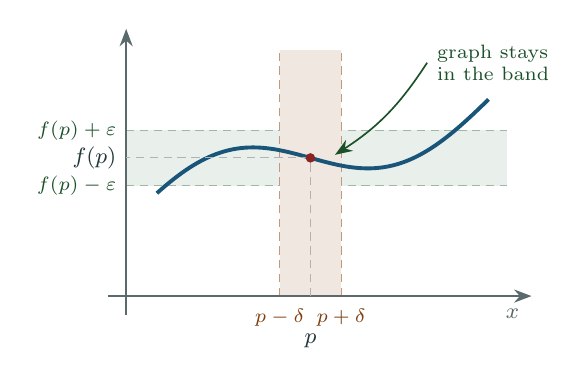
\begin{tikzpicture}[scale=0.78, >={Stealth[length=2.2mm]}]
    % --- bands first (epsilon: green, delta: warm orange) ---
    \fill[proofcolor!10] (0,1.8) rectangle (6.2,2.7);
    \draw[proofcolor!45, densely dashed, thin] (0,1.8) -- (6.2,1.8);
    \draw[proofcolor!45, densely dashed, thin] (0,2.7) -- (6.2,2.7);
    \fill[mAccent!13] (2.5,0) rectangle (3.5,4.0);
    \draw[mAccent!55, densely dashed, thin] (2.5,0) -- (2.5,4.0);
    \draw[mAccent!55, densely dashed, thin] (3.5,0) -- (3.5,4.0);
    % --- axes ---
    \draw[->, mDarkTeal!75, line width=0.9pt]
      (-0.3,0) -- (6.6,0) node[below left=1pt] {\footnotesize $x$};
    \draw[->, mDarkTeal!75, line width=0.9pt] (0,-0.3) -- (0,4.35);
    % --- curve ---
    \draw[defcolor, line width=1.4pt, domain=0.5:5.9, smooth, samples=80]
      plot (\x, {1.2 + 0.35*\x + 0.6*sin(\x*60)});
    % --- dashed guides to (p, f(p)) ---
    \draw[gray!60, densely dashed] (3,0) -- (3,2.25) -- (0,2.25);
    % --- band labels ---
    \node[proofcolor!80!black, left] at (0,2.7) {\scriptsize $f(p) + \varepsilon$};
    \node[proofcolor!80!black, left] at (0,1.8) {\scriptsize $f(p) - \varepsilon$};
    \node[mDarkTeal, left] at (0,2.25) {\footnotesize $f(p)$};
    \node[mAccent!90!black, below] at (2.5,-0.05) {\scriptsize $p - \delta$};
    \node[mAccent!90!black, below] at (3.5,-0.05) {\scriptsize $p + \delta$};
    \node[mDarkTeal, below] at (3,-0.45) {\footnotesize $p$};
    % --- f(p) sits ON the curve: no hole, no jump ---
    \fill[thmcolor] (3,2.25) circle (2.2pt);
    % --- annotation ---
    \draw[->, proofcolor!80!black, semithick]
      (4.9,3.8) node[right, font=\scriptsize, align=left]
      {graph stays\\ in the band}
      to[bend left=12] (3.4,2.3);
  \end{tikzpicture}
  \end{center}

  \begin{hlbox}
  \textbf{Key idea:} the challenge--response game: given the
  \textcolor{proofcolor!80!black}{$\varepsilon$-band}, find a
  \textcolor{mAccent!90!black}{$\delta$-strip} whose graph piece stays
  inside it.
  \end{hlbox}

  \note{
    This diagram shows the definition in action for a real function. The
    blue curve is the graph of "f", and the red dot sits on the curve at
    the point "p" with value "f" of "p": no hole and no jump, in contrast
    to the limit picture of the previous section. The horizontal green
    band is the epsilon challenge: all outputs within epsilon of "f" of
    "p". The vertical orange strip is our delta response: all inputs
    within delta of "p". Continuity at "p" means that no matter how thin
    the green band is, we can choose the orange strip narrow enough that
    the piece of the curve inside the strip stays entirely inside the
    band. Next, two small but important observations.
  }
\end{frame}

% --- Build 1/2 ---
\begin{frame}{Two Observations}
  \begin{remblock}{Observation 1: $f$ must be defined at $p$}
    Continuity at $p$ requires $p \in E$: the value $f(p)$ is part of
    the definition. \\
    (Contrast: for $\lim_{x \to p} f(x)$, we needed $p$ to be a
    \emph{limit point} of $E$, but $p \in E$ was not required.)
  \end{remblock}

  \note{
    First observation. To even ask whether "f" is continuous at "p", the
    function has to be defined at "p"; the point "p" must belong to the
    domain "E", because the value "f" of "p" appears explicitly in the
    definition. Compare this with the limit definition from the previous
    section, where "p" had to be a limit point of "E" but did not have to
    belong to "E" at all. The two definitions have genuinely different
    requirements on "p", and the next observation makes this gap even
    more visible.
  }
\end{frame}

% --- Build 2/2 ---
\begin{frame}{Two Observations}
  \begin{remblock}{Observation 1: $f$ must be defined at $p$}
    Continuity at $p$ requires $p \in E$: the value $f(p)$ is part of
    the definition. \\
    (Contrast: for $\lim_{x \to p} f(x)$, we needed $p$ to be a
    \emph{limit point} of $E$, but $p \in E$ was not required.)
  \end{remblock}

  \begin{remblock}{Observation 2: isolated points are free}
    If $p$ is an \alert{isolated point} of $E$, then \emph{every}
    function $f$ on $E$ is continuous at $p$: choose $\delta$ so small
    that the only $x \in E$ with $d_X(x,p) < \delta$ is $x = p$; then
    $d_Y(f(x), f(p)) = 0 < \varepsilon$.
  \end{remblock}

  \note{
    Second observation. If "p" is an isolated point of "E", then every
    function defined on "E" is automatically continuous at "p", no matter
    how wild it looks elsewhere. The reason is on the slide: we may pick
    delta so small that the only point of "E" within delta of "p" is "p"
    itself. For that single point, the distance between "f" of "x" and
    "f" of "p" is zero, which beats any positive epsilon. So the
    definition is satisfied for free. The interesting case is therefore
    when "p" is a limit point of "E", and that is exactly the case the
    next theorem addresses.
  }
\end{frame}

\begin{frame}{Theorem 4.6: Continuity via Limits}
  \begin{thmblock}{Theorem 4.6}
    In the situation of Definition 4.5, assume also that $p$ is a
    \emph{limit point} of $E$. Then $f$ is continuous at $p$ if and only
    if
    \[
      \lim_{x \to p} f(x) = f(p).
    \]
  \end{thmblock}

  \begin{proofblock}{Proof}
    Compare Definitions 4.1 and 4.5. \qed
  \end{proofblock}

  \vspace{0.3em}
  \begin{hlbox}
  \textbf{Payoff:} all the limit machinery of Section 4.1 (sequences,
  limit laws) now applies to continuity.
  \end{hlbox}

  \note{
    Theorem 4.6 makes the slogan from our motivation precise. When "p" is
    a limit point of "E", continuity at "p" means exactly that the limit
    of "f" of "x" as "x" approaches "p" exists and equals "f" of "p". The
    proof is just a side by side comparison of the two definitions: the
    limit definition quantifies over points "x" different from "p", and
    continuity adds the harmless case "x" equals "p", where the distance
    is zero anyway. The payoff is substantial: every tool we proved about
    limits, in particular the sequential characterization of Theorem 4.2
    and the limit laws of Theorem 4.4, instantly translates into a tool
    about continuity. We will cash this in shortly. First, compositions.
  }
\end{frame}

}

% =============================================================================
% COMPOSITION OF FUNCTIONS
% =============================================================================
{
\usebackgroundtemplate{%
  
\includegraphics[width=\paperwidth,height=\paperheight,keepaspectratio=false]{chapter_04_bg_03.png}%
}
\section{Composition of Functions}

\begin{frame}{Theorem 4.7: Composition of Continuous Functions}
  \begin{thmblock}{Theorem 4.7}
    Suppose $X$, $Y$, $Z$ are metric spaces, $E \subset X$,
    $f \colon E \to Y$, $g \colon f(E) \to Z$, and
    \[
      h(x) = g(f(x)) \qquad (x \in E).
    \]
    If $f$ is continuous at $p \in E$ and $g$ is continuous at $f(p)$,
    then $h$ is continuous at $p$.
  \end{thmblock}

  \vspace{0.3em}
  \hl{$h = g \circ f$ is the \alert{composition} of $f$ and $g$.}

  \vspace{0.3em}
  \begin{hlbox}
  \textbf{Slogan:} a continuous function of a continuous function is
  continuous.
  \end{hlbox}

  \note{
    Our first structural result. We have three metric spaces and two
    functions chained together: "f" maps "E" into "Y", and "g" maps the
    range of "f" into "Z". The composition "h" sends "x" to "g" of "f" of
    "x", and is written "g" circle "f". The theorem says that if "f" is
    continuous at "p", and "g" is continuous at the image point "f" of
    "p", then the composition is continuous at "p". The brief statement
    given in the book is worth memorizing: a continuous function of a
    continuous function is continuous. Let's visualize the setup before
    proving it.
  }
\end{frame}

\begin{frame}{Composition: The Picture}
  \begin{center}
  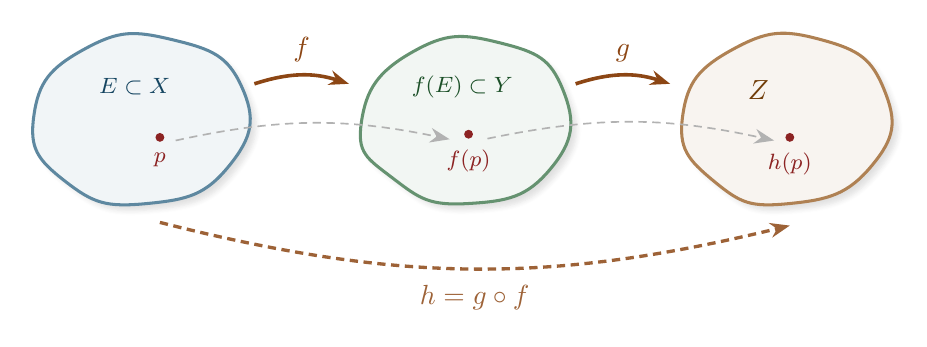
\begin{tikzpicture}[scale=0.8, >={Stealth[length=2.5mm]}]
    % --- Space X with E: organic blob ---
    \draw[defcolor!70, line width=1.1pt, fill=defcolor!6,
          blur shadow={shadow blur steps=6, shadow opacity=12}]
      plot [smooth cycle, tension=0.9] coordinates
      {(-1.8,0.1) (-1.0,1.15) (0.4,1.3) (1.5,0.55) (1.3,-0.7) (0.0,-1.3) (-1.3,-0.95)};
    \node[defcolor!80!black, font=\bfseries\footnotesize] at (-0.2,0.55) {$E \subset X$};
    \fill[thmcolor] (0.2,-0.25) circle (2pt);
    \node[thmcolor, below=2pt] at (0.2,-0.25) {\footnotesize $p$};
    % --- Space Y with f(E): organic blob ---
    \draw[proofcolor!70, line width=1.1pt, fill=proofcolor!6,
          blur shadow={shadow blur steps=6, shadow opacity=12}]
      plot [smooth cycle, tension=0.9] coordinates
      {(3.4,0.0) (4.2,1.1) (5.6,1.25) (6.6,0.5) (6.4,-0.75) (5.1,-1.3) (3.9,-0.9)};
    \node[proofcolor!80!black, font=\bfseries\footnotesize] at (5.0,0.55) {$f(E) \subset Y$};
    \fill[thmcolor] (5.1,-0.2) circle (2pt);
    \node[thmcolor, below=2pt] at (5.1,-0.2) {\footnotesize $f(p)$};
    % --- Space Z: organic blob ---
    \draw[excolor!70, line width=1.1pt, fill=excolor!6,
          blur shadow={shadow blur steps=6, shadow opacity=12}]
      plot [smooth cycle, tension=0.9] coordinates
      {(8.5,0.1) (9.3,1.15) (10.7,1.3) (11.7,0.5) (11.5,-0.7) (10.2,-1.3) (9.0,-0.95)};
    \node[excolor!80!black, font=\bfseries] at (9.7,0.5) {$Z$};
    \fill[thmcolor] (10.2,-0.25) circle (2pt);
    \node[thmcolor, below=2pt] at (10.2,-0.25) {\footnotesize $h(p)$};
    % --- arrows f and g ---
    \draw[->, mAccent, line width=1.3pt] (1.7,0.6) to[bend left=18]
      node[above=1pt, font=\itshape]{$f$} (3.2,0.6);
    \draw[->, mAccent, line width=1.3pt] (6.8,0.6) to[bend left=18]
      node[above=1pt, font=\itshape]{$g$} (8.3,0.6);
    % --- composite h: dashed sweep along the bottom ---
    \draw[->, mAccent!85, line width=1.2pt, densely dashed]
      (0.2,-1.6) to[bend right=14]
      node[below=2pt, font=\itshape]{$h = g \circ f$} (10.2,-1.65);
    % --- gray dashed trace of the point p ---
    \draw[->, gray!60, densely dashed, semithick]
      (0.45,-0.3) to[bend left=12] (4.8,-0.28);
    \draw[->, gray!60, densely dashed, semithick]
      (5.4,-0.27) to[bend left=12] (9.95,-0.3);
  \end{tikzpicture}
  \end{center}

  \vspace{0.3em}
  \begin{hlbox}
  \textbf{Proof strategy:} chain the $\varepsilon$'s --- continuity of
  $g$ produces an intermediate radius $\eta$, which becomes the
  ``$\varepsilon$'' challenge for $f$.
  \end{hlbox}

  \note{
    In the picture, the three shaded regions are the domain "E" inside
    "X" in blue, the range of "f" inside "Y" in green, and the target
    space "Z" in amber. The red points track a single input: "p" is sent
    by "f" to "f" of "p", which is sent by "g" to "h" of "p", following
    the gray dashed trace. The solid orange arrows are the two given
    continuous maps, and the long dashed arrow along the bottom is the
    composition "h". The proof strategy is to chain epsilons. Continuity
    of "g" at the middle point produces an intermediate radius, which we
    call eta. That eta then serves as the epsilon challenge that we hand
    to "f". Let's carry this out.
  }
\end{frame}

% --- Build 1/2 ---
\begin{frame}{Proof of Theorem 4.7}
  \footnotesize
  \begin{proofblock}{Step 1: Use continuity of $g$ at $f(p)$}
    Let $\varepsilon > 0$ be given. There exists $\eta > 0$ such that
    \[
      d_Z(g(y), g(f(p))) < \varepsilon
      \quad \text{if } d_Y(y, f(p)) < \eta \text{ and } y \in f(E).
    \]
  \end{proofblock}

  \note{
    Let epsilon be given; our task is to control the composition. We
    first feed epsilon to the outer function. Since "g" is continuous at
    the point "f" of "p", there is a positive eta such that any point "y"
    of the range of "f" within distance eta of "f" of "p" has its image
    under "g" within epsilon of "g" of "f" of "p". Notice the role
    reversal coming up: this eta, which was an answer extracted from "g",
    now becomes a challenge that we pose to "f".
  }
\end{frame}

% --- Build 2/2 ---
\begin{frame}{Proof of Theorem 4.7}
  \footnotesize
  \begin{proofblock}{Step 1: Use continuity of $g$ at $f(p)$}
    Let $\varepsilon > 0$ be given. There exists $\eta > 0$ such that
    \[
      d_Z(g(y), g(f(p))) < \varepsilon
      \quad \text{if } d_Y(y, f(p)) < \eta \text{ and } y \in f(E).
    \]
  \end{proofblock}

  \begin{proofblock}{Step 2: Use continuity of $f$ at $p$, then chain}
    There exists $\delta > 0$ such that
    \[
      d_Y(f(x), f(p)) < \eta
      \quad \text{if } d_X(x, p) < \delta \text{ and } x \in E.
    \]
    Hence, for such $x$:
    \[
      \boxed{\,d_Z(h(x), h(p)) = d_Z(g(f(x)), g(f(p))) < \varepsilon.\,}
      \qquad \qed
    \]
  \end{proofblock}

  \note{
    Now we feed eta to the inner function. Since "f" is continuous at
    "p", there is a positive delta such that points "x" of "E" within
    delta of "p" are mapped within eta of "f" of "p". Now chain: if "x"
    is within delta of "p", then "f" of "x" is within eta of "f" of "p",
    so by Step 1 its image under "g" is within epsilon of "g" of "f" of
    "p". That is the boxed statement: "h" is continuous at "p". Next
    comes the most elegant result of this section.
  }
\end{frame}

}

% =============================================================================
% THE TOPOLOGICAL CHARACTERIZATION
% =============================================================================
{
\usebackgroundtemplate{%
  
\includegraphics[width=\paperwidth,height=\paperheight,keepaspectratio=false]{chapter_04_bg_04.png}%
}
\section{The Topological Characterization}

\begin{frame}{Theorem 4.8: Continuity via Open Sets}
  \begin{thmblock}{Theorem 4.8}
    A mapping $f$ of a metric space $X$ into a metric space $Y$ is
    continuous on $X$ \alert{if and only if} $f^{-1}(V)$ is open in $X$
    for every open set $V$ in $Y$.
  \end{thmblock}

  \vspace{0.4em}
  \begin{hlbox}
  \textbf{Recall (Definition 2.2):} the \emph{inverse image}
  $f^{-1}(V) = \{x \in X : f(x) \in V\}$.
  \end{hlbox}

  \vspace{0.4em}
  \begin{hlbox}
  \textbf{Why it matters:} no $\varepsilon$, no $\delta$, no distances
  --- continuity becomes a statement about \alert{open sets alone}.
  \end{hlbox}

  \note{
    Here is the highlight of the section. A map "f" from one metric space
    into another is continuous on all of "X" if and only if the inverse
    image of every open set is open. Recall from Definition 2.2 that the
    inverse image of "V" is the set of all points "x" whose image lands
    in "V". Look at what has happened: epsilon, delta, and even the
    distance functions have completely disappeared from the
    characterization. Continuity is revealed as a purely topological
    notion, a statement about open sets alone. This formulation is
    extremely useful, and it will do serious work for us in the sections
    on compactness and connectedness. Let's see the picture behind the
    proof.
  }
\end{frame}

\begin{frame}{Theorem 4.8: The Picture}
  \begin{center}
  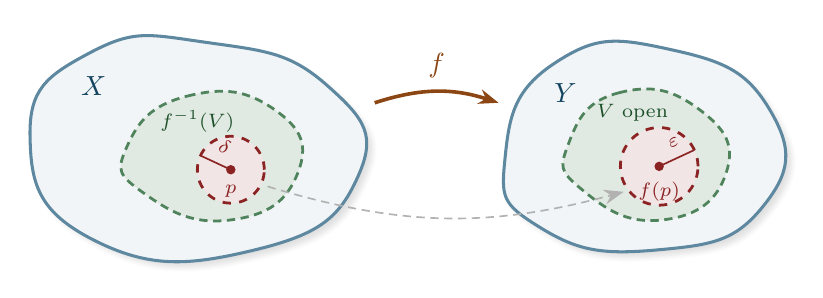
\begin{tikzpicture}[scale=0.85, >={Stealth[length=2.5mm]}]
    % --- Space X: organic blob (widened) ---
    \draw[defcolor!70, line width=1.1pt, fill=defcolor!6,
          blur shadow={shadow blur steps=6, shadow opacity=12}]
      plot [smooth cycle, tension=0.9] coordinates
      {(-2.45,0.2) (-1.55,1.45) (0.2,1.6) (2.0,0.95) (2.45,-0.4) (0.9,-1.5) (-1.5,-1.35)};
    \node[defcolor!80!black, font=\bfseries] at (-1.5,0.95) {$X$};
    % --- f^{-1}(V): open region, dashed rim (enlarged) ---
    \draw[proofcolor!80, line width=1pt, densely dashed, fill=proofcolor!14]
      plot [smooth cycle, tension=0.9] coordinates
      {(-1.0,0.05) (-0.1,0.8) (1.2,0.6) (1.55,-0.35) (0.55,-1.05) (-0.75,-0.65)};
    \node[proofcolor!80!black, font=\scriptsize] at (0.05,0.42) {$f^{-1}(V)$};
    % --- delta ball around p: soft halo + dashed rim + radius ---
    \fill[thmcolor!12] (0.55,-0.3) circle (0.5);
    \draw[thmcolor, dashed, line width=1pt] (0.55,-0.3) circle (0.5);
    \draw[thmcolor, semithick] (0.55,-0.3) --
      node[pos=0.45, above=0.5pt, sloped] {\scriptsize $\delta$} ++(155:0.5);
    \fill[thmcolor] (0.55,-0.3) circle (2pt);
    \node[thmcolor, below=1.5pt, font=\scriptsize] at (0.55,-0.32) {$p$};
    % --- mapping arrow ---
    \draw[->, mAccent, line width=1.3pt] (2.7,0.7) to[bend left=18]
      node[above=1pt, font=\itshape] {$f$} (4.55,0.7);
    % --- Space Y: organic blob (widened) ---
    \draw[defcolor!70, line width=1.1pt, fill=defcolor!6,
          blur shadow={shadow blur steps=6, shadow opacity=12}]
      plot [smooth cycle, tension=0.9] coordinates
      {(4.65,-0.1) (5.4,1.3) (7.1,1.5) (8.6,0.6) (8.5,-0.85) (6.9,-1.5) (5.15,-1.15)};
    \node[defcolor!80!black, font=\bfseries] at (5.55,0.85) {$Y$};
    % --- V: open region, dashed rim (enlarged) ---
    \draw[proofcolor!80, line width=1pt, densely dashed, fill=proofcolor!14]
      plot [smooth cycle, tension=0.9] coordinates
      {(5.6,0.1) (6.35,0.85) (7.55,0.6) (7.95,-0.35) (7.0,-1.05) (5.8,-0.6)};
    \node[proofcolor!80!black, font=\scriptsize] at (6.55,0.55) {$V$ open};
    % --- epsilon ball around f(p) ---
    \fill[thmcolor!12] (6.95,-0.25) circle (0.58);
    \draw[thmcolor, dashed, line width=1pt] (6.95,-0.25) circle (0.58);
    \draw[thmcolor, semithick] (6.95,-0.25) --
      node[pos=0.6, above=0.5pt, sloped] {\scriptsize $\varepsilon$} ++(25:0.58);
    \fill[thmcolor] (6.95,-0.25) circle (2pt);
    \node[thmcolor, below=1.5pt, font=\scriptsize] at (6.95,-0.27) {$f(p)$};
    % --- dashed trace: p is sent to f(p) ---
    \draw[->, gray!60, densely dashed, semithick]
      (1.1,-0.55) to[bend right=16] (6.42,-0.63);
  \end{tikzpicture}
  \end{center}

  \begin{hlbox}
  \textbf{Goal ($\Rightarrow$):} every $p \in f^{-1}(V)$ is an
  \emph{interior point} of $f^{-1}(V)$.
  \end{hlbox}

  \note{
    The picture shows the two spaces side by side, connected by the
    orange arrow for "f". On the left, inside "X", the green region is
    the inverse image of "V", and the point "p" sits in it with a red
    delta ball that continuity will provide. The gray dashed arrow
    carries "p" over to the right, where its image "f" of "p" sits inside
    the open set "V", drawn in green, with a red epsilon ball around it;
    openness of "V" is what provides that ball. For the forward direction
    of the proof, the goal line below the picture is our target: every
    point "p" of the inverse image is an interior point, meaning some
    delta ball around "p" stays inside the inverse image. Let's prove
    exactly that.
  }
\end{frame}

% --- Build 1/2 ---
\begin{frame}{Proof of Theorem 4.8 ($\Rightarrow$)}
  \begin{proofblock}{Setup: continuity $\Rightarrow$ inverse images open}
    Suppose $f$ is continuous on $X$ and $V \subset Y$ is open. Let
    $p \in f^{-1}(V)$, so $f(p) \in V$.
    \begin{itemize}
      \item $V$ open $\;\Longrightarrow\;$ there is $\varepsilon > 0$:
        $y \in V$ whenever $d_Y(f(p), y) < \varepsilon$
    \end{itemize}
  \end{proofblock}

  \note{
    Forward direction. We assume "f" is continuous and take any open set
    "V" in "Y". To show the inverse image is open, pick any point "p" in
    it; by definition, its image "f" of "p" lies in "V". Because "V" is
    open, "f" of "p" is an interior point of "V": there is a positive
    epsilon such that every point of "Y" within epsilon of "f" of "p"
    still belongs to "V". This epsilon is precisely the red ball we drew
    on the right side of the picture. Now continuity enters.
  }
\end{frame}

% --- Build 2/2 ---
\begin{frame}{Proof of Theorem 4.8 ($\Rightarrow$)}
  \begin{proofblock}{Setup: continuity $\Rightarrow$ inverse images open}
    Suppose $f$ is continuous on $X$ and $V \subset Y$ is open. Let
    $p \in f^{-1}(V)$, so $f(p) \in V$.
    \begin{itemize}
      \item $V$ open $\;\Longrightarrow\;$ there is $\varepsilon > 0$:
        $y \in V$ whenever $d_Y(f(p), y) < \varepsilon$
      \item $f$ continuous at $p$ $\;\Longrightarrow\;$ there is
        $\delta > 0$: $d_Y(f(x), f(p)) < \varepsilon$ whenever
        $d_X(x, p) < \delta$
    \end{itemize}
    Hence $d_X(x,p) < \delta \;\Longrightarrow\; f(x) \in V
    \;\Longrightarrow\; x \in f^{-1}(V)$:
    \[
      \boxed{\,p \text{ is an interior point of } f^{-1}(V).\,}
    \]
  \end{proofblock}

  \note{
    Continuity of "f" at "p" with this epsilon hands us a positive delta:
    whenever "x" is within delta of "p", the image "f" of "x" is within
    epsilon of "f" of "p". Combine the two bullets: if "x" is within
    delta of "p", then "f" of "x" is within epsilon of "f" of "p", hence
    "f" of "x" belongs to "V", hence "x" belongs to the inverse image of
    "V". So the entire delta ball around "p" sits inside the inverse
    image, which makes "p" an interior point. Since "p" was arbitrary,
    the inverse image is open. Now for the converse direction.
  }
\end{frame}

% --- Build 1/2 ---
\begin{frame}{Proof of Theorem 4.8 ($\Leftarrow$)}
  \begin{proofblock}{Converse: open inverse images $\Rightarrow$ continuity}
    Suppose $f^{-1}(V)$ is open in $X$ for \emph{every} open $V \subset Y$.
    Fix $p \in X$ and $\varepsilon > 0$. Let
    \[
      V = \{\, y \in Y : d_Y(y, f(p)) < \varepsilon \,\}.
    \]
    \begin{itemize}
      \item $V$ is open (an open ball) $\;\Longrightarrow\;$
        $f^{-1}(V)$ is open, and $p \in f^{-1}(V)$
    \end{itemize}
  \end{proofblock}

  \note{
    Converse direction. Now we assume that the inverse image of every
    open set is open, and we must produce the epsilon delta statement at
    an arbitrary point "p". Fix "p" and a positive epsilon. The trick is
    to make a clever choice of "V": take "V" to be the open ball in "Y"
    of radius epsilon centered at "f" of "p". Open balls are open sets,
    so our hypothesis applies: the inverse image of "V" is open in "X".
    And it certainly contains "p", because the distance from "f" of "p"
    to itself is zero. One more step finishes the proof.
  }
\end{frame}

% --- Build 2/2 ---
\begin{frame}{Proof of Theorem 4.8 ($\Leftarrow$)}
  \begin{proofblock}{Converse: open inverse images $\Rightarrow$ continuity}
    Suppose $f^{-1}(V)$ is open in $X$ for \emph{every} open $V \subset Y$.
    Fix $p \in X$ and $\varepsilon > 0$. Let
    \[
      V = \{\, y \in Y : d_Y(y, f(p)) < \varepsilon \,\}.
    \]
    \begin{itemize}
      \item $V$ is open (an open ball) $\;\Longrightarrow\;$
        $f^{-1}(V)$ is open, and $p \in f^{-1}(V)$
      \item Hence there is $\delta > 0$: $x \in f^{-1}(V)$ whenever
        $d_X(p, x) < \delta$
      \item But $x \in f^{-1}(V) \Rightarrow f(x) \in V \Rightarrow
        d_Y(f(x), f(p)) < \varepsilon$ \hfill $\qed$
    \end{itemize}
  \end{proofblock}

  \note{
    Since the inverse image of "V" is an open set containing "p", the
    point "p" is an interior point of it: there is a positive delta such
    that every "x" within delta of "p" lies in the inverse image. But
    lying in the inverse image means precisely that "f" of "x" belongs to
    "V", which by our choice of "V" means the distance from "f" of "x" to
    "f" of "p" is less than epsilon. That is exactly continuity at "p",
    and since "p" was arbitrary, "f" is continuous on "X". The proof is
    complete. This theorem has an immediate twin for closed sets.
  }
\end{frame}

\begin{frame}{Corollary: Continuity via Closed Sets}
  \begin{thmblock}{Corollary}
    A mapping $f$ of a metric space $X$ into a metric space $Y$ is
    continuous \alert{if and only if} $f^{-1}(C)$ is closed in $X$ for
    every closed set $C$ in $Y$.
  \end{thmblock}

  \begin{proofblock}{Proof}
    A set is closed iff its complement is open, and inverse images
    respect complements:
    \[
      f^{-1}(E^c) = \left[ f^{-1}(E) \right]^c
      \qquad (E \subset Y). \qquad \qed
    \]
  \end{proofblock}

  \note{
    The corollary states that continuity is also equivalent to the
    inverse image of every closed set being closed. The proof rides on
    two facts shown on the slide. First, a set is closed exactly when its
    complement is open. Second, taking inverse images commutes with
    taking complements: the inverse image of a complement is the
    complement of the inverse image. You can check this identity directly
    from the definition of inverse image; it holds for any function
    whatsoever. Combining the two facts converts the open set
    characterization of Theorem 4.8 into the closed set version. Before
    moving on, one warning about a tempting misreading of this theorem.
  }
\end{frame}

\begin{frame}{Caution: Inverse Images, Not Images!}
  \small
  \begin{remblock}{A tempting --- but false --- misreading}
    Theorem 4.8 is about \alert{inverse} images. A continuous $f$ need
    \emph{not} map open sets to open sets!
  \end{remblock}

  \begin{hlbox}
  \textbf{Counterexample:}\\
  $f(x) = x^2$ is continuous on $R$, but
  $f\bigl( (-1, 1) \bigr) = [\,0, 1)$ is \emph{not open} in $R$.
  \end{hlbox}

  \begin{center}
  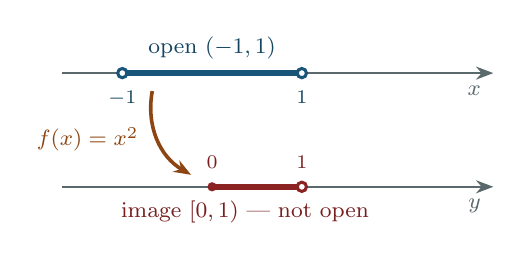
\begin{tikzpicture}[scale=0.76, >={Stealth[length=2.2mm]}]
    % --- domain line ---
    \draw[->, mDarkTeal!75, line width=0.9pt]
      (-2.5,1.2) -- (4.7,1.2) node[below left=1pt] {\footnotesize $x$};
    \draw[defcolor, line width=2pt] (-1.5,1.2) -- (1.5,1.2);
    \fill[white] (-1.5,1.2) circle (2.2pt);
    \draw[defcolor, line width=1.1pt] (-1.5,1.2) circle (2.2pt);
    \fill[white] (1.5,1.2) circle (2.2pt);
    \draw[defcolor, line width=1.1pt] (1.5,1.2) circle (2.2pt);
    \node[defcolor!80!black, below=3pt] at (-1.5,1.2) {\scriptsize $-1$};
    \node[defcolor!80!black, below=3pt] at (1.5,1.2) {\scriptsize $1$};
    \node[defcolor!80!black, font=\footnotesize] at (0,1.62) {open $(-1,1)$};
    % --- image line ---
    \draw[->, mDarkTeal!75, line width=0.9pt]
      (-2.5,-0.7) -- (4.7,-0.7) node[below left=1pt] {\footnotesize $y$};
    \draw[thmcolor, line width=2pt] (0,-0.7) -- (1.5,-0.7);
    \fill[thmcolor] (0,-0.7) circle (2.2pt);
    \fill[white] (1.5,-0.7) circle (2.2pt);
    \draw[thmcolor, line width=1.1pt] (1.5,-0.7) circle (2.2pt);
    \node[thmcolor!85!black, above=3pt] at (0,-0.7) {\scriptsize $0$};
    \node[thmcolor!85!black, above=3pt] at (1.5,-0.7) {\scriptsize $1$};
    \node[thmcolor!85!black, font=\footnotesize] at (0.55,-1.12)
      {image $[0,1)$ --- not open};
    % --- mapping arrow ---
    \draw[->, mAccent, line width=1.3pt] (-1.0,0.9) to[bend right=35]
      node[left=3pt, font=\itshape\footnotesize] {$f(x)=x^2$} (-0.35,-0.5);
  \end{tikzpicture}
  \end{center}

  \note{
    A quick warning before we move on, because this trips up many
    students. Theorem 4.8 talks about inverse images only. It does not
    say that a continuous function maps open sets to open sets, and that
    statement is in fact false. The counterexample is on the slide: the
    squaring function is continuous on the real line, yet it maps the
    open interval from minus 1 to 1, drawn in blue, onto the interval
    from 0 inclusive to 1 exclusive, drawn in red. That image contains
    its left endpoint 0, so it is not open. Continuity pulls open sets
    back to open sets; it does not push them forward. With that warning
    recorded, we turn to the algebra of continuous functions.
  }
\end{frame}

}

% =============================================================================
% ALGEBRA OF CONTINUOUS FUNCTIONS
% =============================================================================
{
\usebackgroundtemplate{%
  
\includegraphics[width=\paperwidth,height=\paperheight,keepaspectratio=false]{chapter_04_bg_05.png}%
}
\section{Algebra of Continuous Functions}

\begin{frame}{Theorem 4.9: Sums, Products, Quotients}
  \begin{thmblock}{Theorem 4.9}
    Let $f$ and $g$ be complex continuous functions on a metric space
    $X$. Then
    \[
      f + g, \qquad fg, \qquad f/g
    \]
    are continuous on $X$ \quad (for $f/g$: assume $g(x) \neq 0$ for all
    $x \in X$).
  \end{thmblock}

  \begin{proofblock}{Proof}
    At \emph{isolated} points of $X$: nothing to prove (Observation 2).
    At \emph{limit} points: combine Theorem 4.4 (limit laws) with
    Theorem 4.6. \qed
  \end{proofblock}

  \note{
    Theorem 4.9 gives us the algebra of continuous functions: if "f" and
    "g" are complex valued continuous functions on "X", then their sum,
    their product, and their quotient are continuous, where for the
    quotient we naturally assume "g" never vanishes on "X". The proof is
    a two line harvest of earlier work. At an isolated point of "X",
    every function is continuous, as we saw in Observation 2, so there is
    nothing to prove. At a limit point, Theorem 4.6 translates continuity
    into a limit statement, and the limit laws of Theorem 4.4 from the
    previous section do all the heavy lifting. The same strategy extends
    to vector valued functions, as we see next.
  }
\end{frame}

% --- Build 1/2 ---
\begin{frame}{Theorem 4.10: Vector-Valued Functions}
  \begin{thmblock}{Theorem 4.10 (a)}
    Let $f_1, \dots, f_k$ be real functions on a metric space $X$, and
    let $\mathbf{f} \colon X \to R^k$ be defined by
    \begin{equation}
      \mathbf{f}(x) = (f_1(x), \dots, f_k(x)) \qquad (x \in X);
      \tag{7}
    \end{equation}
    then $\mathbf{f}$ is continuous \alert{if and only if} each of
    $f_1, \dots, f_k$ is continuous.
  \end{thmblock}

  \vspace{0.3em}
  \hl{$f_1, \dots, f_k$ are the \alert{components} of $\mathbf{f}$.}

  \note{
    Theorem 4.10 handles functions whose values are vectors in "R" "k".
    Part "a" considers "k" real functions on "X", bundled into a single
    map, bold "f", whose value at "x" is the vector with coordinates "f"
    sub 1 of "x" through "f" sub "k" of "x", as shown in equation 7.
    These real functions are called the components of bold "f". The
    statement is an equivalence: the vector valued map is continuous
    exactly when every single component is continuous. So continuity can
    be checked coordinate by coordinate. Part "b" adds the algebra.
  }
\end{frame}

% --- Build 2/2 ---
\begin{frame}{Theorem 4.10: Vector-Valued Functions}
  \begin{thmblock}{Theorem 4.10 (a)}
    Let $f_1, \dots, f_k$ be real functions on a metric space $X$, and
    let $\mathbf{f} \colon X \to R^k$ be defined by
    \begin{equation}
      \mathbf{f}(x) = (f_1(x), \dots, f_k(x)) \qquad (x \in X);
      \tag{7}
    \end{equation}
    then $\mathbf{f}$ is continuous \alert{if and only if} each of
    $f_1, \dots, f_k$ is continuous.
  \end{thmblock}

  \begin{thmblock}{Theorem 4.10 (b)}
    If $\mathbf{f}$, $\mathbf{g} \colon X \to R^k$ are continuous, so are
    $\mathbf{f} + \mathbf{g}$ and $\mathbf{f} \cdot \mathbf{g}$.
  \end{thmblock}

  \vspace{0.2em}
  \begin{hlbox}
  Note: $\mathbf{f} + \mathbf{g}$ maps into $R^k$; the dot product
  $\mathbf{f} \cdot \mathbf{g}$ is a \emph{real} function on $X$.
  \end{hlbox}

  \note{
    Part "b" says that for two continuous mappings of "X" into "R" "k",
    the sum and the dot product are continuous as well. Watch the types
    here: the sum is again a vector valued map into "R" "k", while the
    dot product produces a single real number at each point, so it is a
    real function on "X". The whole theorem rests on one inequality
    relating a vector to its components, which we look at now.
  }
\end{frame}

\begin{frame}{Proof of Theorem 4.10}
  \footnotesize
  \setlength{\abovedisplayskip}{3pt}%
  \setlength{\belowdisplayskip}{3pt}%
  \begin{proofblock}{Proof of (a): one inequality does it all}
    For $j = 1, \dots, k$:
    \[
      |f_j(x) - f_j(y)| \;\leq\; |\mathbf{f}(x) - \mathbf{f}(y)|
      \;=\; \left\{ \sum_{i=1}^{k} |f_i(x) - f_i(y)|^2 \right\}^{1/2}
    \]
    \begin{itemize}
      \item ($\Rightarrow$) $\mathbf{f}$ continuous: left inequality
        forces each $f_j$ continuous (same $\delta$ works)
      \item ($\Leftarrow$) all $f_i$ continuous: right side small when
        each term is small
    \end{itemize}
  \end{proofblock}

  \begin{proofblock}{Proof of (b)}
    Follows from (a) and Theorem 4.9:\\
    The components of
    $\mathbf{f} + \mathbf{g}$ are $f_i + g_i$, and
    $\mathbf{f} \cdot \mathbf{g} = \sum_i f_i g_i$. \qed
  \end{proofblock}

  \note{
    The entire proof of part "a" is the displayed inequality. The
    distance between the vectors bold "f" of "x" and bold "f" of "y" is
    the square root of the sum of the squared component differences, and
    each single component difference is at most that. Reading it left to
    right: if the vector map moves points very little, then every
    component moves even less, so continuity of bold "f" gives continuity
    of each "f" sub "j", with the same delta. Reading it right to left:
    if all "k" components move very little, the sum under the square root
    is small, so the vector moves little too. Part "b" is then free: the
    components of the sum are the sums of components, and the dot product
    is a finite sum of products of real continuous functions, so Theorem
    4.9 applies. Time to harvest some concrete examples.
  }
\end{frame}

}

% =============================================================================
% EXAMPLES
% =============================================================================
{
\usebackgroundtemplate{%
  
\includegraphics[width=\paperwidth,height=\paperheight,keepaspectratio=false]{chapter_04_bg_06.png}%
}
\section{Examples: A Library of Continuous Functions}

\begin{frame}{Examples 4.11: Coordinate Functions}
  \begin{exblock}{The coordinate functions $\phi_i$}
    If $x_1, \dots, x_k$ are the coordinates of $\mathbf{x} \in R^k$,
    the functions
    \begin{equation}
      \phi_i(\mathbf{x}) = x_i \qquad (\mathbf{x} \in R^k)
      \tag{8}
    \end{equation}
    are continuous on $R^k$:
    \[
      |\phi_i(\mathbf{x}) - \phi_i(\mathbf{y})| \leq |\mathbf{x} - \mathbf{y}|
      \quad \Longrightarrow \quad \text{take } \alert{\delta = \varepsilon}
      \text{ in Definition 4.5.}
    \]
  \end{exblock}

  \note{
    Now we build a library of continuous functions, starting from the
    simplest imaginable building block. The coordinate function phi sub
    "i", defined in equation 8, takes a point of "R" "k" and simply reads
    off coordinate number "i". The inequality on the slide says that the
    difference of the corresponding coordinates is at most the distance
    between the points themselves; one coordinate of a vector never
    exceeds the length of the vector. So in Definition 4.5 we can respond to any
    epsilon challenge with delta equal to epsilon itself. These humble
    coordinate readers are sometimes called the coordinate functions,
    and from them we now build all polynomials.
  }
\end{frame}

\begin{frame}{Examples 4.11: Monomials and Polynomials}
  \begin{exblock}{From coordinates to polynomials (via Theorem 4.9)}
    Every \emph{monomial}
    \begin{equation}
      x_1^{n_1} x_2^{n_2} \cdots x_k^{n_k}
      \tag{9}
    \end{equation}
    ($n_1, \dots, n_k$ nonnegative integers) is continuous on $R^k$ ---
    repeated products of the $\phi_i$. Constants are continuous, so
    every \alert{polynomial}
    \begin{equation}
      P(\mathbf{x}) = \Sigma\, c_{n_1 \cdots n_k}
        x_1^{n_1} \cdots x_k^{n_k} \qquad (\mathbf{x} \in R^k)
      \tag{10}
    \end{equation}
    (complex coefficients, finitely many terms) is continuous on $R^k$.
  \end{exblock}

  \note{
    Watch how fast the library grows. A monomial, shown in equation 9, is
    just a finite product of coordinate functions, each possibly repeated
    several times. Since products of continuous functions are continuous
    by Theorem 4.9, repeated application shows every monomial is
    continuous on "R" "k". Constant functions are evidently continuous,
    so constant multiples of monomials are continuous too. Finally, a
    polynomial, shown in equation 10, is a finite sum of such terms, with
    complex coefficients allowed, and sums of continuous functions are
    continuous, again by Theorem 4.9. Conclusion: every polynomial in "k"
    variables is continuous on all of "R" "k".
  }
\end{frame}

\begin{frame}{Examples 4.11: Rational Functions}
  \begin{exblock}{Rational functions}
    Every \alert{rational function} in $x_1, \dots, x_k$ (a quotient of
    two polynomials of the form (10)) is continuous on $R^k$
    \alert{wherever the denominator is nonzero}.
  \end{exblock}

  \vspace{0.4em}
  \begin{hlbox}
  \textbf{Why:} polynomials are continuous + quotient rule of
  Theorem 4.9.
  \end{hlbox}

  \vspace{0.4em}
  \begin{hlbox}
  Example: $\displaystyle \frac{x_1 x_2 - 1}{x_1^2 + x_2^2}$ is
  continuous on $R^2 \setminus \{\mathbf{0}\}$.
  \end{hlbox}

  \note{
    One more application of the quotient rule. A rational function is by
    definition a quotient of two polynomials. Since polynomials are
    continuous everywhere, Theorem 4.9 makes the quotient continuous at
    every point where the denominator is different from zero. As a small
    illustration, the function on the slide, a quotient of two
    polynomials in two variables, is continuous everywhere in the plane
    except at the origin, the single point where its denominator
    vanishes. Our library now contains all polynomials and rational
    functions. Two more entries complete the collection: the absolute
    value, and norms of continuous vector valued maps.
  }
\end{frame}

\begin{frame}{Examples 4.11: The Norm is Continuous}
  \small
  \begin{exblock}{The mapping $\mathbf{x} \to |\mathbf{x}|$}
    The \emph{reverse} triangle inequality:
    \begin{equation}
      \bigl| \, |\mathbf{x}| - |\mathbf{y}| \, \bigr| \leq
      |\mathbf{x} - \mathbf{y}| \qquad (\mathbf{x}, \mathbf{y} \in R^k),
      \tag{11}
    \end{equation}
    so $\mathbf{x} \to |\mathbf{x}|$ is continuous on $R^k$
    (again $\delta = \varepsilon$).

    \textbf{Why:}
    $|\mathbf{x}| = |(\mathbf{x} - \mathbf{y}) + \mathbf{y}|
    \leq |\mathbf{x} - \mathbf{y}| + |\mathbf{y}|
    \;\Longrightarrow\;
    |\mathbf{x}| - |\mathbf{y}| \leq |\mathbf{x} - \mathbf{y}|$
    \, (swap $\mathbf{x} \leftrightarrow \mathbf{y}$).
  \end{exblock}

  \begin{exblock}{Combining with composition (Theorem 4.7)}
    If $\mathbf{f} \colon X \to R^k$ is continuous, then
    $\phi(p) = |\mathbf{f}(p)|$ is continuous real function on $X$.
  \end{exblock}

  \note{
    The final pair of examples. Equation 11, the reverse triangle
    inequality, says the difference of the lengths of two vectors is at
    most the distance between them. The derivation on the slide shows
    the trick: write "x" as "x" minus "y", plus "y". The ordinary triangle
    inequality then bounds the length of "x" by the length of "x" minus
    "y", plus the length of "y". Moving the length of "y" to the left
    side gives one half of equation 11, and swapping the roles of "x"
    and "y" gives the other half. Just as with the coordinate functions,
    delta equals epsilon works, so taking the norm of a vector is a
    continuous operation on "R" "k". And now composition pays off:
    if bold "f" is any continuous map from a metric space "X" into "R"
    "k", then following it with the norm gives the real function phi,
    sending "p" to the length of bold "f" of "p", and Theorem 4.7
    guarantees phi is continuous on "X". One tidy remark, and then we
    summarize.
  }
\end{frame}

}

% =============================================================================
% A SIMPLIFYING REMARK
% =============================================================================
{
\usebackgroundtemplate{%
  
\includegraphics[width=\paperwidth,height=\paperheight,keepaspectratio=false]{chapter_04_bg_07.png}%
}
\section{A Simplifying Remark}

\begin{frame}{Remark 4.12: Forget the Complement}
  \begin{remblock}{Remark 4.12}
    Continuity was defined for $f \colon E \to Y$ with $E \subset X$ ---
    but the \alert{complement of $E$ plays no role} in the definition.
    (The situation was \emph{different} for limits of functions.)
  \end{remblock}

  \vspace{0.4em}
  \begin{hlbox}
  \textbf{Consequence:} we may discard the ambient space and simply
  study \alert{continuous mappings of one metric space into another}
  ($E$ itself is a metric space!).
  \end{hlbox}

  \vspace{0.4em}
  \begin{hlbox}
  This simplifies statements and proofs --- already used in
  Theorems 4.8--4.10, and again in the next section.
  \end{hlbox}

  \note{
    Remark 4.12 cleans up our framework. We defined continuity for a
    function on a subset "E" of a metric space "X", but if you reread
    Definition 4.5, you will notice that the points of "X" outside "E"
    are never mentioned; the complement of "E" plays no role whatever.
    Note that the situation was somewhat different for limits of
    functions, where limit points of "E" inside the ambient space
    mattered. So nothing is lost if we discard the ambient space
    altogether and regard "E", which is a metric space in its own right,
    as the whole domain. From now on we may simply speak of continuous
    mappings of one metric space into another. We already exploited this
    in Theorems 4.8 through 4.10, and the next section on compactness
    will do so constantly.
  }
\end{frame}

}

% =============================================================================
% SUMMARY
% =============================================================================
{
\usebackgroundtemplate{%
  
\includegraphics[width=\paperwidth,height=\paperheight,keepaspectratio=false]{chapter_04_bg_08.png}%
}
\section{Summary}

% --- Build 1/3 ---
\begin{frame}{Summary}
  \footnotesize
  \begin{hlbox}
  \textbf{Key takeaways from this section:}
  \begin{itemize}
    \item \alert{Definition 4.5}: $f$ continuous at $p$:
      $\varepsilon$--$\delta$ control of $d_Y(f(x), f(p))$;\\
      automatic at isolated points
    \item \alert{Theorem 4.6}: at limit points, continuity
      $\iff \lim_{x \to p} f(x) = f(p)$
  \end{itemize}
  \end{hlbox}

  \note{
    Let's review what we covered. We began with Definition 4.5: a
    function is continuous at a point "p" of its domain if for every
    positive epsilon there is a positive delta so that points within
    delta of "p" map to within epsilon of "f" of "p". At isolated points
    the condition holds automatically. Theorem 4.6 then linked this to
    the previous section: at limit points of the domain, continuity says
    precisely that the limit of the function equals its value.
  }
\end{frame}

% --- Build 2/3 ---
\begin{frame}{Summary}
  \footnotesize
  \begin{hlbox}
  \textbf{Key takeaways from this section:}
  \begin{itemize}
    \item \alert{Definition 4.5}: $f$ continuous at $p$:
      $\varepsilon$--$\delta$ control of $d_Y(f(x), f(p))$;\\
      automatic at isolated points
    \item \alert{Theorem 4.6}: at limit points, continuity
      $\iff \lim_{x \to p} f(x) = f(p)$
    \item \alert{Theorem 4.7}: compositions $g \circ f$ of continuous
      functions are continuous
    \item \alert{Theorem 4.8}: $f$ continuous $\iff$ $f^{-1}(V)$ open
      for all open $V$\\
      ($\iff$ $f^{-1}(C)$ closed for all closed $C$)
  \end{itemize}
  \end{hlbox}

  \note{
    Next came the two structural theorems. Theorem 4.7: a continuous
    function of a continuous function is continuous, proved by chaining
    epsilon through an intermediate radius eta. And Theorem 4.8, the gem
    of the section: continuity is equivalent to inverse images of open
    sets being open, with the corollary that it is also equivalent to
    inverse images of closed sets being closed. Continuity is thus a
    purely topological property, with no epsilons in sight.
  }
\end{frame}

% --- Build 3/3 ---
\begin{frame}{Summary}
  \footnotesize
  \begin{hlbox}
  \textbf{Key takeaways from this section:}
  \begin{itemize}
    \item \alert{Definition 4.5}: $f$ continuous at $p$:
      $\varepsilon$--$\delta$ control of $d_Y(f(x), f(p))$;\\
      automatic at isolated points
    \item \alert{Theorem 4.6}: at limit points, continuity
      $\iff \lim_{x \to p} f(x) = f(p)$
    \item \alert{Theorem 4.7}: compositions $g \circ f$ of continuous
      functions are continuous
    \item \alert{Theorem 4.8}: $f$ continuous $\iff$ $f^{-1}(V)$ open
      for all open $V$\\
      ($\iff$ $f^{-1}(C)$ closed for all closed $C$)
    \item \alert{Theorems 4.9--4.10 + Examples 4.11}: sums, products,
      quotients, components; polynomials, rational functions,
      $|\mathbf{x}|$ all continuous
  \end{itemize}
  \end{hlbox}

  \vspace{0.3em}
  \begin{hlbox}
  \textbf{Coming up next:} \emph{Continuity and Compactness} ---
  extreme values, uniform continuity.
  \end{hlbox}

  \note{
    Finally, the algebra and the library. Theorems 4.9 and 4.10 showed
    that sums, products, quotients, and component bundling all preserve
    continuity, and Examples 4.11 cashed these in: coordinate functions,
    monomials, polynomials, rational functions away from their zero
    denominators, and the norm are all continuous. In the next section we
    combine continuity with compactness from Chapter 2. The rewards are
    some of the most useful theorems in analysis: continuous images of
    compact sets are compact, real continuous functions on compact sets
    attain their maximum and minimum, and a new, stronger notion called
    uniform continuity appears. See you in the next episode.
  }
\end{frame}
}

\end{document}
